\documentclass[tikz,svgnames]{standalone}
\usetikzlibrary{matrix,positioning}

\begin{document}
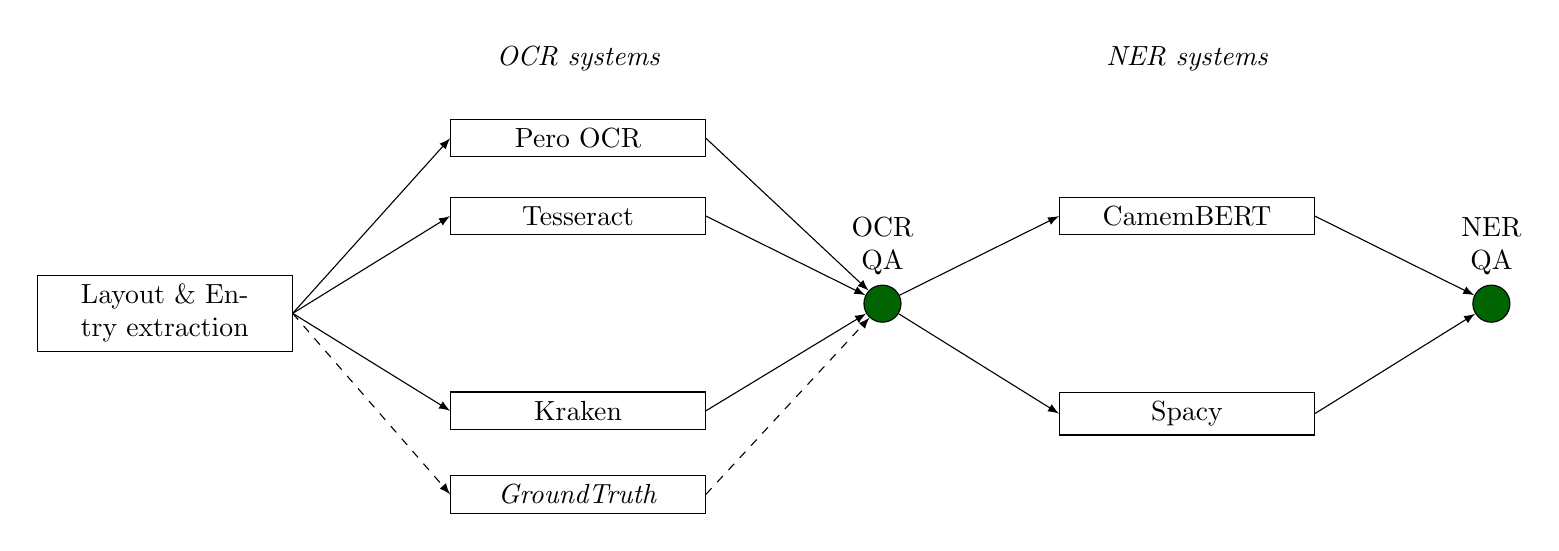
\begin{tikzpicture}
  \tikzset{
    title/.style={every node/.style={draw=none, font=\itshape}},
    qa/.style={circle, fill=DarkGreen, text width=5pt}
  };
  \matrix[matrix of nodes, nodes={draw, align=center, text width=3cm}, column sep=2cm, row sep=.5cm, row 1/.style=title] (A)
  {
    & OCR systems &    & NER systems &    \\
    & |(pero)| Pero OCR        &    &    &    \\
    & |(tess)| Tesseract          &   & |(cam)| CamemBERT &   \\
    |(a)| Layout \& Entry extraction &           & |[qa] (b)|  & & |[qa] (c)|  \\
    & |(kraken)| Kraken   &    & |(spacy)| Spacy       &    \\
    & |(gt)| \emph{GroundTruth}   &    &        &    \\
  };

  \node [above=0cm of b, align=center] {OCR\\ QA};
  \node [above=0cm of c, align=center] {NER\\ QA};

  \begin{scope}[-latex]
{\draw (a.east) -- (pero.west); \draw (pero.east)  -- (b); }
{\draw (a.east) -- (tess.west); \draw (tess.east)  -- (b); }
{\draw (a.east) -- (kraken.west); \draw (kraken.east)  -- (b); }
{\draw[dashed] (a.east) -- (gt.west); \draw[dashed] (gt.east)  -- (b); }

{\draw (b) -- (cam.west);  \draw (cam.east) -- (c); }
{\draw (b) -- (spacy.west);  \draw (spacy.east) -- (c); }

\end{scope}
\end{tikzpicture}

\end{document}